\scanpage{221}
\mspage{220}
\deleted{\unsure{une suite de préschémas}}\inserted{dénombrable (p.ex. de t.f. sur $\mathbb Q$)}, on voit encore que
$\xi_v^{\mathbb Z}\simeq\xi_w^{\mathbb Z}$. En effet, $k$ est réunion filtrante
d'une \uline{suite} $A_i$ de sous-$k_0$-algèbres de type
fini, on peut supposer les morphismes
de transition $\operatorname{Spec}A_j\mathrel{\text{---}}\operatorname{Spec}A_i$
lisses à fibres géom. connexes, de même
pour $X_j\mathrel{\text{---}}X_i$, donc aussi pour $X_{jC}\mathrel{\text{---}}X_{iC}$.
On a des pts $x_i,y_i$ dans $X_{iC}$, s'envoyant
les uns sur les autres par les
morphismes de transition, et grâce à
la lissité et la connexité des fibres,
on voit que les morphismes de
transition $\pi^{\unsure{1|\wedge}}(x_j,y_j)\mathrel{\text{---}}\pi^{\unsure{1|\wedge}}(x_i,y_i)$ sont
surjectifs. Donc $\varprojlim_i\pi^{\unsure{1|\wedge}}(x_i,y_i)\ne\varnothing$,
on gagne.
\figure{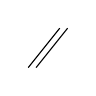
\begin{tikzpicture}\draw (0,0)--(.4,.5);\draw (.1,0)--(.5,.5);\end{tikzpicture}}
Si $k$ pas dénombrable,

2) $E$ \deleted{$k_0$ alg. fermé dans $k$}\inserted{$v$ et $w$ ne coïncident pas sur $E$}.
Alors je \deleted{\unsure{crois}}\inserted{pense} qu'il existe $\alpha$ tel que
\deleted{\unsure{un motif} $M$}
\[
\xi_v^{\mathbb Z}|\mathbb M_\alpha(X)\not\simeq\xi_w^{\mathbb Z}|\mathbb M_\alpha(X).
\]
On peut supposer que $X=\operatorname{Spec}\unsure{E|k}$, $k$ extension
finie de $\mathbb Q$, \deleted{De plus, on peut supposer,
par \unsure{changement de base}, que $k$ \illegible{4} \unsure{sur $\mathbb Q$}.}

\margin{\deleted{\figure{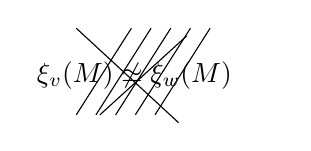
\begin{tikzpicture}
\node[text width=3cm] at (1,0) {$\unsure{\xi_v(M)}\not\simeq\unsure{\xi_w(M)}$};
\foreach \x in {0,.25,.5,.75,1}{\draw (\x,-.5)--(\x+.7,.6);}
\draw (0,.6)--(1.3,-.6);\draw (1.4,.5)--(.3,-.5);
\end{tikzpicture}}}}
